\documentclass{article}

\usepackage{physics} % Handy shortcuts like \pdv, \dd and much more
\usepackage{geometry} % smaller margins, can be adjusted if given arguments
\usepackage{siunitx} % the \si environment for units
\usepackage{mathtools} % The dcases environment, prettier than just cases
\usepackage{tikz} % For drawing picures
\usepackage{wrapfig} % Wrapping text around figures


\title{Exercise 5 - TFY4345 Classical Mechanics}
\date{2020}

\begin{document}
    \maketitle
    \section{Effective potential and scattering center}
        A particle with mass $m$ moves in an attractive potential $V(r)$. Show, on the basis of energy conservation, how the problem can be looked upon as a one-dimensional problem with the effective potential $V_\mathrm{eff}(r)$ What is the condition for the particle to reach the scattering centre, $r=0$? \\ \\
    (Hint: Once setting the condition between $E$ and $V_\mathrm{eff}$, consider the limit where $r \rightarrow 0$.)

    \section{Scattering from a spherical obstacle}
        \begin{wrapfigure}{2}{0.25\textwidth}
            \vspace{-1cm}
            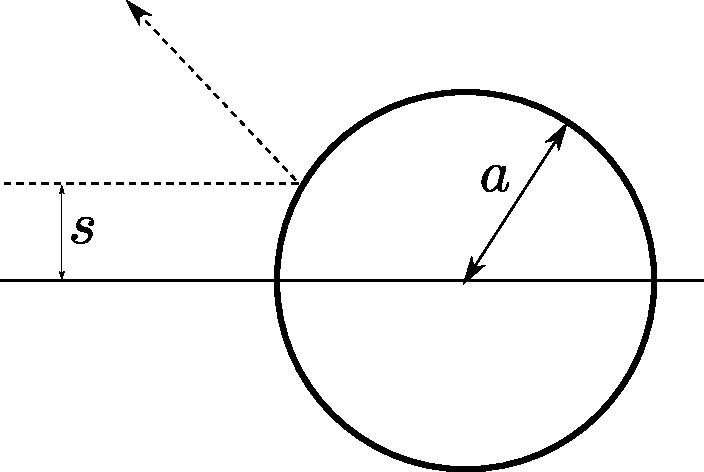
\includegraphics[width=0.24\textwidth]{figures/figure_1.pdf}
            \vspace{-1cm}
        \end{wrapfigure}
        (a) Find the differential cross section $\sigma(\theta)$ for scattering against a hard sphere of radius $a$. Notice when the impact parameter is $s = 0$ the scattering angle is $\theta = \pi$, and when $s > a$ the scattering angle is $\theta = 0$ (no scattering). \\ \\
        (Hint: Use simple geometrical considerations to find a relation between the impact parameter $s$ and the scattering angle $\theta$.) \\ \\
        (b) Calculate the total cross section $\sigma$. Why is the final expression for $\sigma$ reasonable?

    \section{Scattering by an attractive hard sphere}
        A hard sphere has radius $a$. For $r > a$, the sphere yields a Kepler potential $V(r) = - k/r$, where $k>0$. Particles coming in from infinity have mass $m$ and original velocity $v_0$. The part of the particles having impact parameter $s \leq s_{\mathrm{max}}$ will hit the sphere's surface. Find $s_{\mathrm{max}}$, and the corresponding "effective" scattering cross section $\sigma_\mathrm{eff} = \pi s_{\mathrm{max}}^2$. \\ \\
        (Hint: Consider the conservation of energy and angular momentum.)

    \section{Average energies in the Kepler problem}
        (a) The solution to the Kepler problem (particle in a central fore potential $V = -k/r$) is given by the following expression (in polar coordinates):
        \begin{equation*}
            r = \frac{p}{1 + \varepsilon \cos(\theta)}.
        \end{equation*}
        Here, $p$ and $\varepsilon$ are constants (whose definitions can be found in the compendium, chapter 4). Use the expression defining $p$ and $\varepsilon$ to show that the total energy is 
        \begin{equation*}
            E = - \frac{k}{2p}(1 - \varepsilon^2),
        \end{equation*}
        Use the viral theorem and find the average kinetic energy $\expectationvalue{T}$, and the average potential energy $\expectationvalue{V}$. \\ \\
        (b) The average potential energy an be calculated as the average over one orbit period:
        \begin{equation*}
            \expval{V} = \frac{1}{t_p} \int_0^{t_p} \dd t V,
        \end{equation*}
        where $t_p$ is the total orbital period (time for one complete orbit). Find $\expval{V}$ by direct calculation of this integral (not using the viral theorem). Equation 4.35 in the compendium tells us that the period is given by
        \begin{equation*}
            t_p = \frac{2m}{\ell} \pi a b = \frac{2 \pi m}{\ell } \frac{p}{1 - \varepsilon^2} \frac{p}{\sqrt{1 - \varepsilon^2}} = \frac{2 \pi m}{\ell^2} \frac{1}{(1 - \varepsilon^2)^{3/2}}.
        \end{equation*}
        Hint 1: change variable of integration from $t$ to $\theta$\\
        Hint 2: the residue method (E. Kreyzig, 9th ed., chapter 16.4) gives
        \begin{equation*}
            \int_0^{2\pi} \frac{\dd \theta}{1 + \varepsilon \cos(\theta)} = \frac{2 \pi}{\sqrt{1 - \varepsilon^2}}.
        \end{equation*}
        Hint 3: 
        \begin{equation*}
            \int_0^{2\pi} \frac{\dd \theta \cos(\theta)}{(1 + \varepsilon \cos(\theta))^2} = - \dv{\varepsilon} \int_0^{2\pi} \frac{\dd \theta}{1 + \varepsilon \cos(\theta)}  
        \end{equation*}
        (c) The average kinetic energy is:
        \begin{equation*}
            \expval{T} = \frac{1}{t_p} \int_0^{t_p} \dd t\, T = \frac{1}{t_p} \int_0^{t_p} \dd t \, \frac{1}{2} m \left(\dv{\mathbf{r}}{t}\right)^2.
        \end{equation*}
        Find $\expval{T}$ by direct calculation of this integral. \\ \\
        Hint: Do the integral by parts, and use Newton's equation
        \begin{equation*}
            m \dv[2]{\mathbf{r}}{t} = - \nabla V = - \frac{k}{r^3} \mathbf{r}.
        \end{equation*}
        Note also that the integration (by parts) is take over a full period where the particle has returned back to its starting position.


\end{document}

 